\usetikzlibrary{patterns}

\section{Спецификация данных}
...
\section{Функциональные требования}
\noindent\indent Разрабатываемая система должна:
\begin{enumerate}
  \item Определять силы и моменты сил действующие на парус в каждый момент времени
  \item Определять углы оптимального управления
\end{enumerate}
\section{Проект}
\subsection{Средства реализации}
\noindent\indent При разработке использовался язык программирования C/C++,
как основной язык разработки системы моделирования <<Sputnix Satellite Modeller>>.
\subsection{Модули и алгоритмы}
\subsubsection{Прогнозирование оптимального <<положения>>}
\noindent\indent Предполагаем, что мы имеем возможность считать углы оптимального
управления в каждый момент времени для максимизации подынтегральной функции за довольно
малые промежутки времени. Тем самым, с течением времени, мы получим ряды, состоящие
из оптимальных углов и тех, что имеются на самом деле:
\begin{equation}
  \begin{aligned}
    &\{\theta_{t_i}\}_{i=\overline{1,N}} = \theta_{t_0}, \theta_{t_1}, ..., \theta_{t_N}, \\
    &\{\hat{\theta}_{t_i}\}_{i=\overline{1,N}} = \hat{\theta}_{t_0}, \hat{\theta}_{t_1}, ..., \hat{\theta}_{t_N}, \\
    &\{\phi_{t_i}\}_{i=\overline{1,N}} = \phi_{t_0}, \phi_{t_1}, ..., \phi_{t_N} \\
    &\{\hat{\phi}_{t_i}\}_{i=\overline{1,N}} = \hat{\phi}_{t_0}, \hat{\phi}_{t_1}, ..., \hat{\phi}_{t_N}, \\
  \end{aligned}
\end{equation}
здесь $\hat{\theta}_{t_i}$, $\hat{\phi}_{t_i}$ -- оптимальные углы управления аппаратом,
высчитанные для момента времени $t_i$; $\theta_{t_i}$, $\phi_{t_i}$ -- углы, которыми
ориентирована система в момент времени $t_i$.\par
  В таком случае, для наилучшей оптимизации функционала, необходимо, чтобы
аппарат мгновенно менял свою ориентацию на наиболее оптимальную, что в условиях
существования внешних возмущающих моментов сил и собственного вращающего момента
спутника трудно достижимо.\par
  Однако, имея выборку уже вычисленных значений, возможно приближенно спрогнозировать
наиболее оптимальные угловые коэффициенты, которые должен будет принять аппарат
через некоторый промежуток времени $\Delta t$ и сделать управляющую функцию изменения
углов более плавной для большей эффективности системы автоматической ориентации КА.\par
  Пусть $\vec{W} = (\phi, \theta)^T$ -- вектор углов. Разложим значение данного вектора
в точке $t_{k+1}$ через ряд Тейлора в точке $t_{k}$:
\begin{equation} \label{eq:parialWEquatation}
  \vec{W}_{t_{k+1}} = \vec{W}_{t_{k}}
  + \frac{\partial}{\partial t}\vec{W}_{t_{k}} \cdot (t_{k+1} - t_{k})
  + \frac{\partial^2}{\partial t^2}\vec{W}_{t_{k}} \cdot (t_{k+1} - t_{k})^2
  + o(|t_{k+1} - t_{k}|^3)
\end{equation}\par
  Так как нам известно оптимальное значение углов, которое <<мгновенно>> необходимо
придать в каждой точке отсчета, значит, мы знаем <<мгновенную>> скорость, которую
будет пытаться придать система стабилизации КА:
\begin{equation}
  \frac{\partial}{\partial t}\vec{W}_{t_{k}} = \hat{\vec{W}}_{t_{k}} - \vec{W}_{t_{k}},
\end{equation}\par
  Также возможно получить приближенное значение дифференциала второго порядка путем
усреднения значений пересчетов между ближайшими узлами расчета:
\begin{equation}
  \frac{\partial^2}{\partial t^2}\vec{W}_{t_{k}} = \frac{1}{2}\left[
    \frac{\frac{\partial}{\partial t}\vec{W}_{t_{k+1}} - \frac{\partial}{\partial t}\vec{W}_{t_{k}}}{t_{k+1} - t_{k}}
    +
    \frac{\frac{\partial}{\partial t}\vec{W}_{t_{k}} - \frac{\partial}{\partial t}\vec{W}_{t_{k-1}}}{t_{k} - t_{k-1}}
  \right]
\end{equation}\par
  Тем самым мы получаем возможность предсказывать приближенное значение углов,
ориентирующих аппарат в заданный момент времени.\par
  Однако, есть ограничения на данную конструкцию. Как описывалось выше, управляющие
углы зависят не только от времени, но и от взаимного положения КА, Земли и Солнца,
тем самым разложение в ряд Тейлора примет следующий вид:
\begin{equation} \label{eq:FullWEquatation}
  \vec{W}_{t_{k+1,\vec{K}_{k+1}}} = \vec{W}_{t_{k},\vec{K}_{k}}
  + \left[
    \frac{\partial}{\partial t}\vec{W}_{t_{k},\vec{K}_{k}} \cdot (t_{k+1} - t_{k})
  + \frac{\partial}{\partial \vec{K}_k}\vec{W}_{t_{k},\vec{K}_{k}} \cdot (\vec{K}_{k+1} - \vec{K}_{k})
  \right]
  + o(||(t_{k+1} - t_{k}, \vec{K}_{k+1} - \vec{K}_{k})||^2),
\end{equation}\par
  В таком случае, для упрощения модели (\ref{eq:FullWEquatation}) до вида (\ref{eq:parialWEquatation})
необходимо ввести некоторые ограничения для более приближенного решения, к примеру:
\begin{equation} \label{eq:FullWApprox}
  \begin{aligned}
    &||(t_{k+1} - t_{k}, \vec{K}_{k+1} - \vec{K}_{k})||^2 - ||t_{k+1} - t_{k}||^2 < \delta,\\
    &||\frac{\partial}{\partial \vec{K}_k}\vec{W}_{t_{k},\vec{K}_{k}}|| < \epsilon,
  \end{aligned}
\end{equation}
где $\epsilon$ и $\delta$ -- некоторые специально подобранные константы.\par
  С целью уменьшения количества расчетов, возможна замена условий из (\ref{eq:FullWApprox})
на более жесткое:
\begin{equation}
  ||\vec{K}_{k+1} - \vec{K}_{k}|| < \zeta,
\end{equation}
где $\zeta$ -- специально подобранный коэффициент.
\subsubsection{Аппроксимация управляющих углов}
\noindent\indent Имея выборку найденных управляющих углов и углов ориентации
аппарата возможно применить метод сглаживания управляющих углов.\par
  Рассмотрим график изменения одного из углов в момент времени $t_{n} \rightarrow t_{n+1}$ :
\begin{figure}[!h]%{r}{0pt}
  \centering
  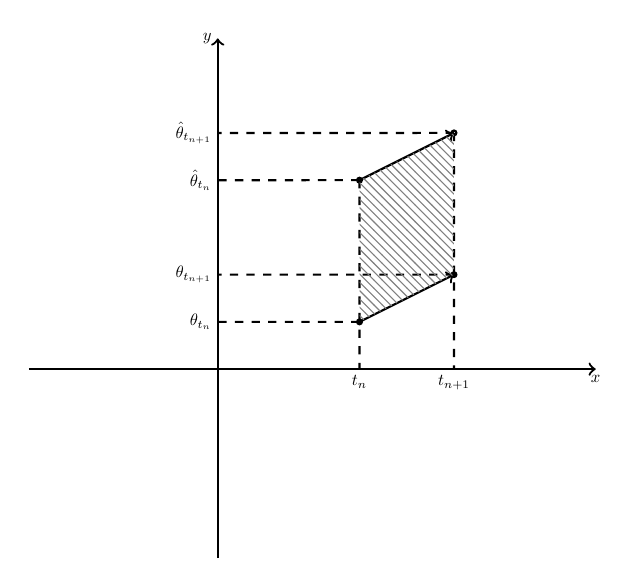
\begin{tikzpicture}[thick,scale=0.6, every node/.style={transform shape}]
    % coordinate system
    \coordinate (O) at (0,0);
    \coordinate (Y) at (0,7);
    \coordinate (X) at (8,0);

    \draw[thick, ->] (-4, 0) -- (X) node[below] {$x$};
    \draw[thick, ->] (0, -4) -- (Y) node[left] {$y$};

    % coordinates of points
    \coordinate (W0) at (3, 1);
    \coordinate (W1) at (5, 2);
    \coordinate (HatW0) at (3, 4);
    \coordinate (HatW1) at (5, 5);

    \node[draw, circle, inner sep=1pt, fill] at (W0) {};
    \node[draw, circle, inner sep=1pt, fill] at (W1) {};

    \node[draw, circle, inner sep=1pt] at (HatW0) {};
    \node[draw, circle, inner sep=1pt] at (HatW1) {};

    \draw[dashed] (W0) -- (0, 1) node[left] {$\theta_{t_{n}}$};
    \draw[dashed] (W1) -- (0, 2) node[left] {$\theta_{t_{n+1}}$};

    \draw[dashed] (HatW0) -- (0, 4) node[left] {$\hat{\theta}_{t_{n}}$};
    \draw[dashed] (HatW1) -- (0, 5) node[left] {$\hat{\theta}_{t_{n+1}}$};

    \draw[dashed] (HatW0) -- (3, 0) node[below] {$t_{n}$};
    \draw[dashed] (HatW1) -- (5, 0) node[below] {$t_{n+1}$};

    % vectors
    \draw[->] (W0) -- (W1);
    \draw[->] (HatW0) -- (HatW1);

    % fill area
    \path[pattern=north west lines, pattern color=gray] (W0) -- (W1) -- (HatW1) -- (HatW0);

  \end{tikzpicture}
  \caption{Изменение управляющего угла и угла ориентации}
  \label{fig:DeltaWHatW}
\end{figure}\par
  Из графика видно, что после попытки изменения углов ориентации, в следующем узле
остчета, уже необходимо менять новую ориентацию используя новые управляющие углы.
Чтобы минимизировать изменения управляющих углов и углов ориентации, воспользуемся
применим конструкцию <<PID>>-регулятора, вида:
\begin{equation}
  u^{t_{n+1}} =
      K_p \cdot s^{t_{n+1}}_{t_n}
    + K_i \cdot \sum\limits_{k=0}^{n} s^{t_{k+1}}_{t_k} (t_{k+1} - t_k)
    + K_d \cdot \frac{s^{t_{n+1}}_{t_n} - s^{t_{n}}_{t_{n-1}}}{t_{k+1} - t_k},
\end{equation}
где $u^{t_{n+1}}_{t_n}$ -- функция управления в момент времени $t_{n+1}$;
$s^{t_{n+1}}_{t_n}$ -- невязка.\par
  В качестве функции невязки необходимо взять такую функцию, чтобы площадь фигуры,
образуемой на графике (\ref{fig:DeltaWHatW}) стала минимальной.\par
  Возьмем в качестве невязки саму площадь фигуры, образуемой отрезками прямых,
проходящих через точки $\theta_{t_{n}}$, $\theta_{t_{n+1}}$ и $\hat{\theta}_{t_{n}}$,
$\hat{\theta}_{t_{n+1}}$:
\begin{equation}\label{eq:SumBtwLines}
  \begin{aligned}
    & s^{t_{n+1}}_{t_n} = \int\limits_{t_n}^{t_{n+1}} |l_1 - l_2| dt, \\
    & l_1: y = \frac{\theta_{t_{n+1}} - \theta_{t_{n}}}{t_{n+1} - t_{n}} \cdot (t - t_{n}),\\
    & l_2: y = \frac{\hat{\theta}_{t_{n+1}} - \hat{\theta}_{t_{n}}}{t_{n+1} - t_{n}} \cdot (t - t_{n}),\\
  \end{aligned}
\end{equation}
где $l_1$, $l_2$ -- уравнения прямых, проходящих через данные точки.\par
  Упростим выражение (\ref{eq:SumBtwLines}), подставив уравнения прямых:
\begin{equation}
  \begin{aligned}
    & s^{t_{n+1}}_{t_n} = \int\limits_{t_n}^{t_{n+1}} \left|\frac{(\hat{\theta}_{t_{n+1}} - \hat{\theta}_{t_{n}}) - (\theta_{t_{n+1}} - \theta_{t_{n}})}{t_{n+1} - t_{n}}\right| \cdot |t - t_{n}| dt, \\
    & s^{t_{n+1}}_{t_n} = \left|\frac{(\hat{\theta}_{t_{n+1}} - \hat{\theta}_{t_{n}}) - (\theta_{t_{n+1}} - \theta_{t_{n}})}{t_{n+1} - t_{n}}\right| \cdot \int\limits_{t_n}^{t_{n+1}} |t - t_{n}| dt, \\
    & s^{t_{n+1}}_{t_n} = \left|\frac{(\hat{\theta}_{t_{n+1}} - \hat{\theta}_{t_{n}}) - (\theta_{t_{n+1}} - \theta_{t_{n}})}{t_{n+1} - t_{n}}\right| \cdot \int\limits_{t_n}^{t_{n+1}} |t - t_{n}| dt, \\
    & s^{t_{n+1}}_{t_n} = \left|\frac{(\hat{\theta}_{t_{n+1}} - \hat{\theta}_{t_{n}}) - (\theta_{t_{n+1}} - \theta_{t_{n}})}{t_{n+1} - t_{n}}\right| \cdot \left[ \frac{t^2_{n+1} - t^2_{n}}{2} - t_{n}(t_{n+1} - t_{n}) \right], \\
    & s^{t_{n+1}}_{t_n} = \left|\frac{(\hat{\theta}_{t_{n+1}} - \hat{\theta}_{t_{n}}) - (\theta_{t_{n+1}} - \theta_{t_{n}})}{t_{n+1} - t_{n}}\right| \cdot \frac{(t_{n+1} - t_{n})^2}{2}, \\
    & s^{t_{n+1}}_{t_n} = \left|(\hat{\theta}_{t_{n+1}} - \hat{\theta}_{t_{n}}) - (\theta_{t_{n+1}} - \theta_{t_{n}})\right| \cdot \frac{|t_{n+1} - t_{n}|}{2}, \\
  \end{aligned}
\end{equation}
\subsubsection{Оптимизация на больших участков}
\noindent\indent Для нахождения оптимального управляющего углового функционала,
для некотором интервале времени, необходимо решить задачу оптимизации нелинейной
интегральной функции (\ref{eq:IntMaxFullEq}). Для этого, представим угловую функцию
в следующем виде:
\begin{equation}
  \begin{aligned}
    & \vec{W}(t) = (\phi(t), \theta(t))^T, \\
    & \vec{W}(t) = \vec{W}_0 + \vec{W}_1 t + \frac{1}{2}\vec{W}_2 t^2, \\
    & \vec{W}_0, \vec{W}_1, \vec{W}_2 \in [-\pi, \pi],
  \end{aligned}
\end{equation}
где $\vec{W}_0$, $\vec{W}_1$, $\vec{W}_2$ -- коэффициенты, которые необходимо найти.\par
  Возможно несколько подходов к решению данной задачи, в частности, метод наименьших
квадратов, генетический алгоритм, алгоритм Нелдера-Мида и градиентный метод.
